\chapter{CONCLUSION}
\section{Summary of the Results}

Section 2.2 has clearly justified the choice of mean as a viable pre-processing technique for handling missing values in the Pima Indian diabetes dataset. Hence, the comparison between the constructed classification models was done after handling the missing values with mean. The results obtained is tabulated in Table 5.1.

\newline
\begin{center}
\begin{tabular}{|c|c|c|c|c|}
\hline
\textbf{Parameter} &	\textbf{ID3} & \textbf{CART} & \textbf{C4.5} &	\textbf{ANN} \\
\hline
Accuracy & 79.87 & 78.57 & 77.27 & 81.17\\
\hline
Sensitivity &	70.21 &	65.95 &	62.96 &	76.59\\
\hline
Specificity &	84.11 &	84.11 &	85 & 83.17\\
\hline
Precision	& 66 &	64.58 &	69.39 &	66.66\\
\hline
\end{tabular}
\end{center}
\captionof{table}{Evaluation metrics for all models after pre-processing with mean}

\begin{figure}[h]
\centering
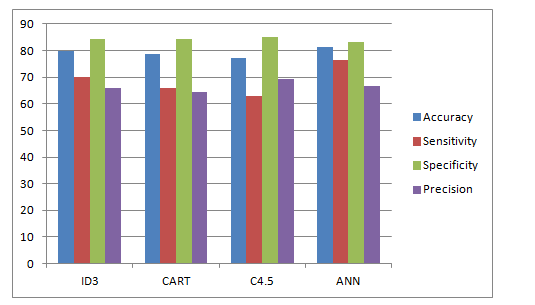
\includegraphics[scale=1.0]{evalmetall.PNG}
\caption{\label{fig:subBDDs1}Evaluation metrics for every model after
preprocessing with mean}
\end{figure}
\pagebreak

The bar chart visualization of the obtained results in Figure 5.1, shows that the ANN model has given the highest accuracy ahead of ID3, which emerged as the best decision tree model considering three evaluation metrics. It has also shown a significant increase of 6.38\% in the Sensitivity value when compared to ID3, which again had the best Sensitivity among the constructed decision trees. The Specificity value for ANN has slightly decreased (by 0.94\%) when compared to ID3. With respect to precision, it was C4.5 which gave the highest value of 69.39\%, ahead of ANN’s 66.66\%. Though, ANN has given slightly lower Specificity and Precision scores in comparison, it has clearly outperformed the other classification models, considering the other two metrics. Hence it can be rightly concluded that ANN has emerged as the best model when compared to the three decision tree variants, from an overall perspective.

\section{Future Work}
\begin{enumerate}
    \item The proposed project can be extended into an interactive application, say a Mobile or Web Application. The system can take values for various parameters as input and feed the constructed ANN. The output from Neural Network will correspond to either non-diabetic or diabetic (ie Outcome = 0 or 1). Hence, the predicted value will help the user know if he/she is classified as diabetic or not based on the parameters. 
    \item The subjects used for the Pima Indian Diabetes dataset are all women who are at least 21 years of age. Hence this data can be augmented with samples belonging to the male gender and people who are lesser than 21, which renders more generalization for the data as well as results. Moreover, all the diabetic patients in this dataset are affected by Type-2 diabetes. Hence, the same models can be constructed for a dataset pertaining to patients affected by Type-1 diabetes.
\end{enumerate}